\documentclass[lettersize,journal]{IEEEtran}
\usepackage{amsmath,amsfonts}
\usepackage{algorithmic}
\usepackage{algorithm}
\usepackage{array}
\usepackage[caption=false,font=normalsize,labelfont=sf,textfont=sf]{subfig}
\usepackage{textcomp}
\usepackage{stfloats}
\usepackage{url}
\usepackage{verbatim}
\usepackage{graphicx}
\usepackage{cite}
\usepackage{xcolor}
\usepackage{amsthm}
\usepackage{svg}
\usepackage{booktabs}
\usepackage{siunitx}
\captionsetup[subfloat]{font=normalsize, labelfont=rm} % 使用 Roman 字体
\sisetup{
	scientific-notation = true,
	round-mode = figures,
	round-precision = 2
}



\hyphenation{op-tical net-works semi-conduc-tor IEEE-Xplore}
% updated with editorial comments 8/9/2021
% 定义推论环境
\newtheorem{corollary}{Corollary}
\newtheorem{proposition}{Proposition}
\newtheorem{lemma}{Lemma}  % 定义lemma环境
\begin{document}
	
	\title{Optimal Power Allocation for Dual-Hop Hybrid Power Line/Wireless System}
	
	\author{Zhen Wang, Wei Peng,~\IEEEmembership{Senior Member, ~IEEE,}
		% <-this % stops a space
		\thanks{This paper was produced by the IEEE Publication Technology Group. They are in Piscataway, NJ.}% <-this % stops a space
		\thanks{Manuscript received April 19, 2021; revised August 16, 2021.}}
	
	% The paper headers
	\markboth{IEEE Transactions on Communications,~Vol.~XX, No.~X, Month~2024}%
	{Wang \MakeLowercase{\textit{et al.}}: Optimal Power Allocation for Dual-Hop Hybrid Power Line/Wireless System}
	
	\IEEEpubid{0000--0000/00\$00.00~\copyright~2021 IEEE}
	% Remember, if you use this you must call \IEEEpubidadjcol in the second
	% column for its text to clear the IEEEpubid mark.
	
	\maketitle
	
	\begin{abstract}
		This paper addresses the optimal power allocation problem in a dual-hop hybrid power line/wireless system (DH-HPWS). Each medium uses OFDM technology for signal transmission, and the relay and destination receiver nodes employ Maximum Ratio Combining (MRC) for signal reception. Due to different constraints, the problem is formulated as two distinct optimization problems: the sum power constraint (SPC) and the source-relay power constraint (SRPC). We provide the mathematical formulation of the problem and propose optimal subcarrier matching and power allocation algorithms under both power constraints, aimed at maximizing the achievable data rate. An interesting finding is that the subcarrier matching methods are opposite between the same link with two media and different links. Furthermore, numerical analysis compares the proposed algorithm with others, evaluating the performance and effectiveness of each approach. The comparison with Interior Point (IP)-based algorithms demonstrates the optimality of the proposed approach. Additionally, under the SRPC condition, optimal subcarrier matching helps improve the efficiency of the optimal power allocation algorithm and simplifies the system structure.
	\end{abstract}
	
	\begin{IEEEkeywords}
		Power allocation, subcarrier matching, dual-hop, hybrid systems, wireless communication, power line communication
	\end{IEEEkeywords}
	
	\section{Introduction}
	\label{sec:intro}
	\IEEEPARstart{A}{s} the demand for communication network capacity continues to rise due to the explosive growth of the Internet of Things (IoT) and the Internet of Everything (IoE) \cite{6714496, 8076908, 9902969}, telecom industries and research institutions are continuously advancing data communication technologies to meet these growing needs.
	
	Power line communication (PLC) \cite{8760230, 8995538, DEOLIVEIRA2022107168} and wireless communication (WLC) \cite{9887796, 9961877, 9900419} are the two most extensively studied communication technologies in the literature. PLC leverages existing power networks to transmit data, offering low cost and easy deployment \cite{doi:10.1049/PBPO132E, 10.5555/3055710}. However, its signal propagation is influenced by factors such as impedance mismatch, time-varying behavior of the load, frequency-selective attenuation, and power noise from large pulses caused by load dynamics \cite{article, electronics8091022, 9239378}. Wireless communication, on the other hand, faces challenges like signal attenuation, line-of-sight issues, sensitivity to co-channel interference, and limited spectrum resources \cite{7467419, 920866, 10.5555/559977}. Despite these challenges, both media have distinct advantages in their respective application scenarios, making their combination a promising approach to enhancing communication system performance.
	
	The integration of Hybrid Powerline Wireless Communication System (HPWS) that use both powerline and radio frequency (RF) channels in indoor environments offers several key advantages. Firstly, it ensures a more stable and reliable network connection. While PLC systems excel at maintaining connectivity through walls and floors, WLC systems often experience interference and signal degradation when faced with such physical barriers. By combining both technologies, users can leverage the diversity they offer, enhancing the overall network performance \cite{6575217}, \cite{5502091}. Additionally, the integration of PLC and WLC systems can significantly extend coverage and connectivity options. In areas where WLC signals are weak or absent—particularly in spaces with thick concrete walls or metal barriers that obstruct wireless signals—PLC systems can fill the coverage gaps. The seamless handover between the two systems guarantees uninterrupted connectivity for users.Another important benefit of integrating PLC and WLC systems is the enhanced security it provides. Users can take advantage of the security features offered by both systems, strengthening the overall network defense. Furthermore, research indicates that leveraging diversity between the systems can improve physical layer security (PLS) in indoor environments \cite{BORBOR201996}. Aimed at inspiring researchers and practitioners, \cite{10298615}  presented comprehensive and multidimensional discussions of the potential and benefits of integrating power line and wireless communication systems to enhance data communication in both indoor and outdoor environments.
	
	However, in both wireless and powerline communication systems, long-distance transmissions often suffer from significant signal attenuation. To address this limitation, relay-assisted communication systems have emerged as an effective solution. By introducing relays, signals can be amplified and retransmitted, significantly extending the range and improving the reliability of long-distance communications. In both PLC and wireless communication networks, relays help mitigate the effects of signal attenuation and interference, ensuring stable and efficient data transmission even over longer distances.
	
	\cite{8187635} formulated the hybrid power line/wireless single-relay channel model and analyzed its suitability for improving data communication in terms of ergodic achievable data rates and outage probabilities.\cite{8421566} investigated the benefits that energy harvesting (EH) can offer to increase energy efficiency in hybrid power line/wireless data communication systems.\cite{7973142} analyzed an wireless sensors and PLC relaying system that improves the capacity and reliability for IoT networks. 
	
	Moreover, Power allocation is a widely recognized and fundamental topic in the fields of PLC and WLC research.	Furthermore,The studies in \cite{9122404} and \cite{9665745} respectively investigated optimal power allocation to maximize the achievable data rate and minimizing the average bit error probability (BEP) in HPWS. Subsequently, \cite{9815250} investigated subcarrier arrangement to optimize the aforementioned algorithms. Considering non-hybrid systems, \cite{5071270} addressed the optimal subcarrier matching and power allocation problem in OFDM multi-hop systems. However, there has been no research conducted on the optimal power allocation problem for DH-HPWS so far.
	
	Therefore, To fill the gaps mentioned above, this paper considers the hybrid nature and resource constraints of HPWS and investigates the optimal subcarrier matching and power allocation algorithms for dual-hop HPWS, with the goal of maximizing the achievable data rate. The contributions of this paper can be summarized as follows:
	\begin{itemize}
		\item The system architecture of the DH-HPWS is presented, in which both the source and relay nodes employ OFDM technology for information transmission, while the destination node adopts MRC for signal reception.
		\item A comprehensive analysis of the relationship between power allocation and the achievable data rate in the DH-HPWS system is conducted. Considering both the total power constraint and the individual power constraints at the source and relay nodes, the mathematical formulations of the problems are provided. Optimal power allocation and subcarrier matching algorithms are proposed, along with theoretical proofs of their optimality.
		\item The proposed methods are compared with conventional approaches, and the optimality of the algorithms is validated through IP-based algorithms. The correctness of the subcarrier matching algorithm is demonstrated from both theoretical and mathematical perspectives. Additionally, an analysis of systems with and without optimal subcarrier matching is conducted, highlighting the performance benefits achieved through optimal matching.
	\end{itemize}
	
	Our major findings are as follows:
	
	\begin{itemize}
		\item The optimal subcarrier matching strategy assigns subcarriers with high normalized signal-to-noise ratio (nSNR) at the source to those with high-nSNR at the relay, and similarly for low-nSNR subcarriers. Under individual power constraints at the source and relay nodes, if one node has surplus power during optimal power allocation, the other node's power allocation follows the classical water-filling solution independently.
		\item Under optimal subcarrier matching, the achievable data rate obtained by the proposed algorithm approaches that achieved by applying water-filling independently at both the source and relay. As the overall available power increases, the achievable rate gain from subcarrier matching gradually diminishes. Furthermore, under separate power constraints, the achievable rate gain from subcarrier matching reaches its maximum when the available powers at the source and relay are approximately equal.
	\end{itemize}
		
	The rest of this paper is organized as follows. Section \ref{sec:system} presents the system model and the formulation of the optimization problem. Section \ref{spc} discusses the optimization problem under total power constraint and provides the optimal power allocation algorithm. Section \ref{srpc} addresses the optimization problem under individual power constraints at the source and relay, along with the corresponding optimal power allocation algorithm. Section \ref{na} presents simulation results to validate the proposed algorithms, and finally, Section \ref{conl} concludes the paper.
	

	
	\section{SYSTEM ARCHITECTURE AND PROBLEM FORMULATION}
	\label{sec:system}
	Consider an IoT system with the following characteristics:
	
	The DH-HPWS model is shown in Fig. \ref{fig_sys}, where the signal is transmitted from the source node (\( S \)) to the relay node (\( R \)), and then from the relay node to the destination node (\( D \)). Dashed lines represent the wireless medium (subscript 1), while solid lines represent the power line medium (subscript 2). It is assumed that the distance from \( S \) to \( D \) is relatively long, with no direct link. Additionally, the relay node operates in a half-duplex mode, and both the relay (\( R \)) and destination (\( D \)) nodes employ MRC technology for signal reception. Furthermore, in this model, the power line and wireless branches operate in different frequency bands, and the total frequency bandwidth is assumed to be equal to \( B_w \). Therefore, both media can simultaneously transmit the same information to enhance medium diversity.
		\begin{figure}[!t]
		\centering
		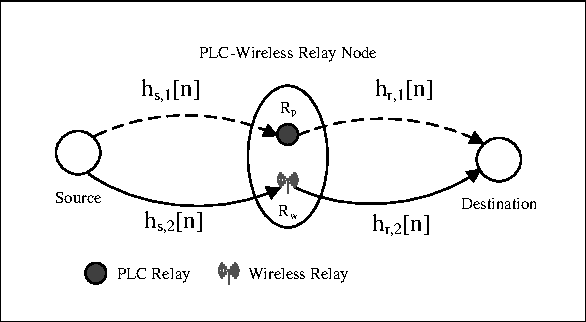
\includegraphics[width=3.5in, trim=10 1 10 1, clip]{system.pdf}
		\caption{System architecture of an dual-hop hybrid power line/wireless system.}
		\label{fig_sys}
	\end{figure}
	
	To cover a wider range of scenarios, we aim to explore a general hybrid system model to derive conclusions applicable to a general number of media. Therefore, the hybrid system consisting of two parallel media is defined as a linear time-varying (LTV) system. It is assumed that the time interval during which data communication occurs is smaller than the shortest coherence time of all parallel channels, allowing the system to be modeled as a linear time-invariant (LTI) system within this time interval. Additionally, in this model, the power line and wireless branches operate in different frequency bands, both employing OFDM technology with \( N \) subcarriers for signal transmission, with the total frequency bandwidth being equal to \( B_w \). Therefore, both media can simultaneously transmit the same information, enhancing the diversity of the media.

	\begin{equation}		
		Y_m^{k,i} = \sqrt {p_m^{k,i}} H_m^{k,i}X_m^{k,i} + Z_m^{k,i}
	\end{equation}
	Where \( H_m^{k,i} \), \( Z_m^{k,i} \), and \( p_m^{k,i} \) represent the channel frequency response, noise, and power for the \( k \)-th medium and \( i \)-th subchannel of the \( m \)-link, where \( m \in \{SR, RD\} \) represents the SR or RD link, \( k \in \{1, 2\} \) representing the wireless and power line media , respectively, and \( i \in \{1, 2, \dots, N\} \).
	
	As described in \cite{9122404}, the normalized received nSNR is defined as:
	
	\begin{equation}
		\overline \gamma  _m^{k,i} \buildrel \Delta \over = |H_m^{k,i}{|^2}/{p_{Z_m^{k,i}}}
	\end{equation}
	
	In this paper, considering the subcarrier arrangement across different transmission media and the subcarrier matching along the link, Fig.~\ref{fig:SR} illustrates the link of a single OFDM symbol from \( S \) to \( R \).
	
	\begin{figure*}[htbp]
		\centering
		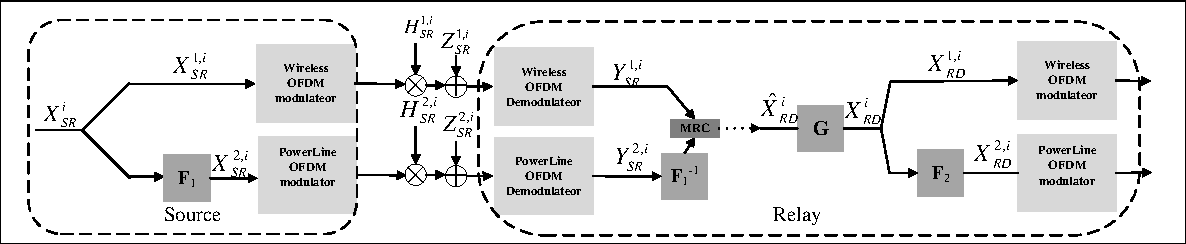
\includegraphics[width=\linewidth, trim=10 1 10 1, clip]{fig2.pdf}
		\caption{OFDM symbol transmission diagram showing subcarrier arrangement and matching from source to relay.}
		\label{fig:SR}
	\end{figure*}
	
	In the figure, \( \mathbf{F}_1 \), \( \mathbf{F}_2 \), and \( \mathbf{G} \) are \( N \times N \) permutation matrices, where \( \mathbf{F}_1 \) and \( \mathbf{F}_2 \) are used for subcarrier permutation, and \( \mathbf{G} \) is used for subcarrier matching. Each of these matrices has one and only one entry equal to 1 in every row and every column, with all other entries being zero.
	
	Let \( X_{\mathrm{SR}}^i \)  and \( X_{\mathrm{RD}}^i \) denote the \( i \)-th symbol, where \( i \in \{1, 2, \dots, N\} \), after QAM/PSK modulation, mapped onto the \( i \)-th subchannel. In the figure, we have the relationships \( X_{\mathrm{SR}}^{2, f_1(i)} = X_{\mathrm{SR}}^i \), \( X_{\mathrm{RD}}^{ 2, f_2(i)} = X_{\mathrm{RD}}^i \), and \( X_{\mathrm{RD}}^ {g(i)} = \hat{X}_{\mathrm{RD}}^i \).
	
	Note that the operations at the relay node \( R \) after MRC, such as decoding and re-encoding, are omitted in this figure.Since MRC is employed, the received signal-to-noise ratios (SNRs) from different branches are coherently combined at the receiver. The power-line communication (PLC) and wireless media can thus be treated as an equivalent unified medium. Accordingly, the received signal-to-noise ratio (SNR) of the \( i \)-th subchannel over the equivalent medium of link \( m \) is defined as follows:
	
	\begin{equation}
		\gamma _m^i = p_m^{1,i}\overline \gamma  _m^{1,i} + p_m^{2,{f_j}(i)}\overline \gamma  _m^{2,{f_j}(i)}
	\end{equation}
	Let \( \gamma_m^i \) denote the received SNR of the \( i \)-th subchannel over the equivalent medium of link \( m \), where \( i \in \{1, 2, \dots, N\} \) and \( \{m, j\} \in \{\{\mathrm{SR}, 1\}, \{\mathrm{RD}, 2\}\} \). Each subchannel transmits over a bandwidth of \( \Delta f \), resulting in a total system bandwidth of \( B_w = \Delta f \times N \).
	
	The subcarrier spacing \( \Delta f \) is typically chosen to be smaller than the minimum coherence bandwidth among all channels~\cite{9122404}, ensuring frequency-flat fading per subchannel. The total bandwidth \( B_w \) is determined by regulatory requirements. In HPWS, \( B_w \) is usually defined by PLC regulations, which tend to impose stricter bandwidth constraints than wireless standards.
	
	Assuming a sampling rate of \( 2B_w \), the achievable rate of the equivalent medium for link \( m \) is given by:
	\begin{equation}
		{R_m} = \frac{{{B_w}}}{N}\sum\limits_{i = 1}^N {{{\log }_2}(1 + \gamma _m^i)} 
	\end{equation}
	Since a half-duplex DF relay is used, the rate of a single subchannel in the system is determined by the lower rate between the SR and RD links. The overall system rate is the sum of the rates of each subchannel. Therefore, the overall system rate is given by:
	
	\begin{equation}
		\begin{aligned}
			R_{\text{global}} &= \frac{B_w}{N} \sum\limits_{i=1}^N \min \left( \log_2 \left( 1 + \gamma_{\text{SR}}^i \right), \right. \\
			& \left. \log_2 \left( 1 + \gamma_{\text{RD}}^{g(i)} \right) \right)
		\end{aligned}
		\label{eq:rate}
	\end{equation}
	
	
	A current challenge is how to find the optimal power allocation that maximizes \( R_{\text{global}} \). Currently, two constraint conditions are considered:
	
	A.  SPC, i.e., \(\sum\limits_{m,k,i} {p_m^{k,i}}  \le {P_t}\), where \( P_{t} \) is the maximum allowable total power.
	
	B. SRPC, i.e., the transmission power at the source and relay is constrained such that \( \sum\limits_{k,i} p_{\text{SR}}^{k,i} \leq P_S \) and \( \sum\limits_{k,i} p_{\text{RD}}^{k,i} \leq P_R \), where \( P_S \) and \( P_R \) represent the maximum allowable transmission powers at the source and relay, respectively.
	
	The first constraint aims to achieve the theoretical maximum rate, while the second constraint takes into account the different power limits at the source and relay nodes. The second constraint is more suitable for practical scenarios, especially when the only source of power at the relay node comes from the energy harvested from the signals received at the \( R \) node.
	
	Now, let \( \zeta = \{A, B\} \) represent the constraints \( A \) or \( B \). The optimization problem can be expressed as follows:
	
	\begin{equation}
		\begin{aligned}
			C_\zeta &= \max \frac{B_w}{N} \sum\limits_{i=1}^N \min \Bigg( \log_2 \left( 1 + \gamma_{\text{SR}}^i \right), \\
			& \quad \log_2 \left( 1 + \gamma_{\text{RD}}^{g(i)} \right) \Bigg) \\
			\text{subject to:} \quad & \sum\limits_{m,k,i} p_m^{k,i} \leq P_t, \quad \text{for } \zeta = \text{A} \\
			& \sum\limits_{k,i} p_{\text{SR}}^{k,i} \leq P_S, \quad \sum\limits_{k,i} p_{\text{RD}}^{k,i} \leq P_R, \quad \text{for } \zeta = \text{B} \\
			& p_m^{k,i} \geq 0, \quad \forall m,k,i, \quad \text{for } \zeta = \text{A or B}
		\end{aligned}
	\end{equation}
	The above formulation considers that the same information is transmitted over both wireless and wired links within the same link, while taking into account the subcarrier permutation across different media and subcarrier matching across different links. Finding the optimal power allocation scheme for the above problem is crucial for the DH-HPWS scheme. Therefore, the following question arises: "How should the power be allocated to maximize the overall achievable rate, considering the subcarrier permutation between different media and the subcarrier matching across different links?"
	
	In the following Sections 3 and 4, this paper will provide solutions for both Constraint A and Constraint B.
	
	\section{Sum Power Constraint}
	\label{spc}
	Under the total power constraint, the optimization equation is as follows:
	\begin{equation}
		\label{eq:7}
		\begin{aligned}
			C_A &= \max \frac{B_w}{N} \sum_{i=1}^N \min \Bigl( \log_2 \left( 1 + \gamma_{\text{SR}}^i \right), \\
			& \log_2 \left( 1 + \gamma_{\text{RD}}^{g(i)} \right) \Bigr) \\
			\text{subject to:} \quad & \sum_{m,k,i} p_m^{k,i} \leq P_t, \\
			& p_m^{k,i} \geq 0, \quad \forall m,k,i
		\end{aligned}
	\end{equation}
	
	
	
	Directly solving this equation is challenging, but the previous research provides valuable insights for this paper. In \cite{9815250}, the optimal solution for an HPWS system without relays is presented, demonstrating that in the optimal allocation, only the maximum N channels from both wireless and powerline media can be selected. The following will prove that this theorem can be extended to a DH-HPWS under the SPC.
	
	\begin{proposition}
		 In a DH-HPWS, if the number of subchannels for both wireless and powerline media is N, to achieve the maximum achievable rate, power allocation should still select the N channels with the highest nSNR for each link under the SPC. 
	\end{proposition}
	\begin{proof}[By contradiction]
		Assume that the SR link achieves optimal performance without selecting the $N$ subchannels with maximal normalized nSNR under power allocation $\mathbf{p} = (p_1,...,p_N)$. Let $\mathcal{A}$ denote the selected subchannel set, and define $a \in \mathcal{A}$ as the subchannel with minimal nSNR:
		\begin{equation}
			\overline \gamma_{\mathrm{SR}}^{a} = \min_{i \in \mathcal{A}} \overline \gamma_{\mathrm{SR}}^{i}.
		\end{equation}
		
		By the pigeonhole principle, there exists an unselected subchannel $b \notin \mathcal{A}$ satisfying:
		\begin{equation}
			\overline \gamma_{\mathrm{SR}}^{b} > \overline \gamma_{\mathrm{SR}}^{a}.
		\end{equation}
		
		We construct an improved subchannel set $\mathcal{A}' = (\mathcal{A}\setminus\{a\}) \cup \{b\}$ and corresponding power allocation $\mathbf{p}'$:
		\begin{align}
			p'_b &= p_a, \quad p'_a = 0, \\
			p'_i &= p_i, \quad \forall i \in \mathcal{A}\setminus\{a\}.
		\end{align}
		
		The resulting rate improvement is:
		\begin{equation}
			\Delta R = \frac{B_w}{N} \left[ \log_2(1 + p_a\gamma_{\mathrm{SR}}^{b}) - \log_2(1 + p_a\gamma_{\mathrm{SR}}^{a}) \right] > 0,
		\end{equation}
		where the strict inequality follows from $\gamma_{\mathrm{SR}}^{b} > \gamma_{\mathrm{SR}}^{a}$.
		
	    From \eqref{eq:rate}, we have $R_{\mathrm{global}}'  \geq R_{\mathrm{global}}$. The same argument holds for the RD link, thus proving the theorem for DH-HPWS. \qedhere
	\end{proof}
	
	From the above inference, in the SR and RD links, select the \(N\) sub - channels with the top - \(N\) largest \(n\text{SNR}\) values from the \(2N\) sub - channels of each link, and these \(N\) sub - channels are equivalent to an equivalent medium, which simplifies the optimization equation to:
	\begin{equation}
		\begin{aligned}
			C_A =& \max \frac{B_w}{N} \sum_{i = 1}^N \min \left( \log_2 \left(1 + p_{SR}^i \overline{\gamma}_{SR}^i \right), \right. \\
			& \left. \log_2 \left(1 + p_{RD}^i \overline{\gamma}_{RD}^{g(i)} \right) \right) \\
			\text{subject to} & \quad \sum_{m,k,i} p_m^{k,i} \leq P_{\text{Total}}, \\
			& \quad p_m^{k,i} \geq 0 \quad \forall m,k,i
		\end{aligned}
	\end{equation}
	Where \(\overline{\gamma}_{SR}^i\) (\(\overline{\gamma}_{RD}^i\)), with \(i \in \{1, 2, 3, \cdots, N\}\), represents the \(i\) - th sub - channel of the equivalent medium in the link from \(S\) to \(R\) (from \(R\) to \(D\)). The simplified equation is similar to the one solved by WenYi Wang \cite{wenyi2008}, which will assist us in solving the above equation. The time complexity of Mo's algorithm is \( O(N \log N) \), and that of Wang's algorithm is also \( O(N \log N) \). Therefore, the overall time complexity of Algorithm 1 is \( O(N \log N) \).
	
	Proposed Algorithm:
	\begin{algorithm}[H]
		\caption{Power Allocation Algorithm for Maximizing Achievable Rate of DH-HPWS under SPC}\label{alg:alg1}
		\begin{algorithmic}
			\STATE \textbf{Input:} nSNR values of subchannels over SR and RD links for both power-line and wireless media
			\STATE \textbf{Output:} Power allocation for each subchannel
			\STATE
			\STATE \textbf{Begin}
			\STATE \quad - Initialize all subchannel power to 0
			\STATE \quad - Use Mo's algorithm to select the top $N$ subchannels with the highest nSNR from both SR and RD links as the equivalent medium
			\STATE \quad - Use Wang's algorithm to allocate power to the selected $N$ subchannels on the SR and RD links
			\STATE \textbf{End}
		\end{algorithmic}
		\label{alg1}
	\end{algorithm}
	
	\section{Source Relay Power Constraint}
	\label{srpc}
	Under individual power constraints at the \(S\) and \(R\) nodes, it can similarly be shown that Mo's theorem also holds for the DH-HPWS. Therefore, as in the case of the total power constraint, the optimization problem can be simplified as follows:
	\begin{equation}
		\begin{aligned}
			\max \quad  C =& \sum_{i=1}^{N} \min \left( \ln\left(1 + p_{SR}^i \, \overline{\gamma}_{SR}^i \right), \right. \\
			& \left. \ln\left(1 + p_{RD}^i \, \overline{\gamma}_{RD}^{g(i)} \right) \right) \\
			\text{subject to} \quad 
			& \sum_{i=1}^{N} p_{SR}^i \leq P_S, \\
			& \sum_{i=1}^{N} p_{RD}^i \leq P_R, \\
			& p_{SR}^i \geq 0, \quad p_{RD}^i \geq 0, \quad \forall i
		\end{aligned}
		\label{eq:separate_power_constraints}
	\end{equation}
	Note that all subsequent references to subcarriers pertain to those of the equivalent medium.
	
	To gain a clearer understanding of the system capacity, we utilize the max-flow min-cut theorem [12], which provides an upper bound on the channel capacity as follows:
	\begin{equation}
		{C_{up}} = \min (\hat {R}_{SR},\hat {R}_{RD})
		\label{eq:15}
	\end{equation}
	Here, \( \hat{R}_{SR} \) denotes the maximum achievable rate at the source node, and \( \hat{R}_{RD} \) denotes the maximum achievable rate at the relay node. Both are obtained using the well-known water-filling algorithm. Without loss of generality, we assume that \( \hat{R}_{SR} \leq \hat{R}_{RD} \)
	
	In the following, we address this optimization problem in two parts:  
	A. Deriving the optimal subcarrier pairing, i.e., determining the optimal \( g(i) \);  
	B. Proposing the optimal power allocation algorithm.  
	  
	It is important to note that these two components are independent — the solution to one does not affect the other.
	
	\subsection{Optimal Subcarrier Pairing}
	
	Consider the case where the OFDM system has only two subcarriers.
	
	\begin{proposition}[Two-Subcarrier OFDM Case]
	\label{prop:main}
		In an OFDM system with only two subcarriers, the subcarrier with the higher nSNR should be paired with the subcarrier that also has the higher nSNR. Similarly, the subcarrier with lower nSNR should be paired with the one having lower nSNR.
	\end{proposition}
	
	\begin{proof}
		See Appendix A. \qed
	\end{proof}
	\begin{corollary}[N-Subcarrier OFDM Case]
		In an OFDM system with \( N \) subcarriers, let the nSNRs of the source and relay be denoted as \( \overline{\gamma}_{SR}^{1} \leq \cdots \leq \overline{\gamma}_{SR}^{N} \) and \( \overline{\gamma}_{RD}^{1} \leq \cdots \leq \overline{\gamma}_{RD}^{N} \), respectively. Then, the optimal subcarrier pairing is the sequential matching, where \( \overline{\gamma}_{SR}^{i} \) is paired with \( \overline{\gamma}_{RD}^{i} \) for \( \forall i \in \{1, \dots, N\} \).
		\label{corollary:2}
	\end{corollary}
	
	\begin{proof}
		Let the nSNRs of the source and relay for the \( N \) subcarriers be denoted as \( \overline{\gamma}_{SR}^{1} \leq \cdots \leq \overline{\gamma}_{SR}^{N} \) and \( \overline{\gamma}_{RD}^{1} \leq \cdots \leq \overline{\gamma}_{RD}^{N} \), respectively, where \( i \in \{1, \dots, N\} \).
		
		Assume that the matching between subcarriers \( i \) and \( j \) is such that \( \overline{\gamma}_{SR}^{i} \) is paired with \( \overline{\gamma}_{RD}^{j} \), where \( j \neq i \). According to Proposition 1, if \( \overline{\gamma}_{SR}^{i} \) is paired with \( \overline{\gamma}_{RD}^{j} \), then there must exist two pairs of subcarriers that violate Proposition 1, specifically the pairs \( (\overline{\gamma}_{SR}^{i}, \overline{\gamma}_{RD}^{i}) \) and \( (\overline{\gamma}_{SR}^{j}, \overline{\gamma}_{RD}^{j}) \), which contradicts the optimal matching rule stated in Proposition 1. Therefore, the only valid matching is to pair \( \overline{\gamma}_{SR}^{i} \) with \( \overline{\gamma}_{RD}^{i} \) for \( \forall i \in \{1, \dots, N\} \).
		
		Thus, the optimal subcarrier matching is the sequential pairing as proposed, where each \( \overline{\gamma}_{SR}^{i} \) is paired with \( \overline{\gamma}_{RD}^{i} \) for \( \forall i \in \{1, \dots, N\} \).
		\(\square\)
	\end{proof}
	Thus, the optimal subcarrier matching for the system is divided into two steps:
	\begin{enumerate}
		\item Sort and label the subcarriers for both the source and relay nodes;
		\item Pair subcarriers with the same index, transmitting the same information.
	\end{enumerate}
	
	Based on Corollary~\ref{corollary:2}, the above matching is the optimal subcarrier pairing. The next section introduces the optimal power allocation algorithm.
	\subsection{Optimal Power Allocation}
	
	In the previous section, the optimal subcarrier pairing scheme was derived. This subsection presents the optimal power allocation algorithm for \( N \) subcarriers under source and relay power constraints. It is important to note that the optimal power allocation algorithm is independent of the optimal subcarrier pairing scheme.
	
	Assuming \( P_S \) and \( P_R \) are the power constraints for the \(S\)) and \(R\) nodes, respectively, but without considering subcarrier pairing, this section divides the relationship between \( P_S \) and \( P_R \) into two cases.
	\begin{enumerate}
		\item If \( P_R \) is large enough to satisfy the water-filling condition for the \(S\), the channel capacity reaches the upper bound.
		\item If \( P_R \) does not satisfy the \(S\) water-filling condition.
	\end{enumerate}
	Note that by "satisfying," it is meant that the \(S\) uses the water-filling algorithm, and the \(R\) also has a power allocation such that \( R_{RD}^{i} = R_{SR}^{i} \) for \( \forall i \in \{1, 2, \dots, N\} \), and the relay power constraint is satisfied, i.e., \( \sum_{i} p_{RD}^i \leq P_R \).
	
	In the first case, the optimal power allocation is achieved by applying the water-filling algorithm to \(S\). The second case, however, is more complex. Next, this section will focus on analyzing the optimal power allocation algorithm for the second case.
	
	Before presenting the optimal power allocation algorithm, there is a consensus that needs to be clarified.
	\begin{proposition}
		In the case of allowing power residuals, the optimal power allocation results in equal subcarrier rates for the matched subcarriers, i.e., \( R_{RD}^{i} = R_{SR}^{i} \), for \( \forall i \in \{1, \dots, N\} \).
	\end{proposition}
	\begin{proof}
		If there \( \exists i \in \{1, \dots, N\} \)  such that \( R_{SR,i} \neq R_{RD,i} \), without loss of generality, assume \( R_{SR}^i < R_{RD}^i \). Then, reducing \( p_{RD}^i \) such that \( R_{SR}^i = R_{RD}^i \) will not affect the system capacity.
	\end{proof}
	
	Before presenting the optimal power allocation algorithm, we establish a key property: in the case of allowing power residuals, the optimal power allocation results in equal subcarrier rates for the matched subcarriers, i.e., \( R_{RD}^{i} = R_{SR}^{i} \), for \( \forall i \in \{1, \dots, N\} \). This follows from the fact that if \( R_{SR}^i < R_{RD}^i \) for any subcarrier \( i \), we can reduce \( p_{RD}^i \) to make the rates equal without affecting system capacity.
	
	Based on this observation, we can focus only on the source node's channel capacity. This introduces an additional constraint that relates the power allocation at both nodes:
	\begin{equation}
		p_{SR}^i \overline{\gamma}_{SR}^i = p_{RD}^i \overline{\gamma}_{RD}^i .  
		\label{eq:16}
	\end{equation}
	
	With this constraint, the optimization problem in \eqref{eq:separate_power_constraints} can be reformulated as:
	\begin{equation}
		\begin{aligned}
			C = & \min - \sum_{i=1}^{N} \ln \left( 1 + p_{SR}^i \overline{\gamma}_{SR}^i \right) \\
			\text{subject to} \quad & p_{SR}^i \overline{\gamma}_{SR}^i = p_{RD}^i \overline{\gamma}_{RD}^i, \quad \forall i, \\
			& \sum_{i} p_{SR}^i \leq P_S, \\
			& \sum_{i} p_{RD}^i \leq P_R, \\
			& p_{SR}^i \geq 0, \quad \forall i.
		\end{aligned}
		\label{eq:opt_power_allocation}
	\end{equation}
	
	Note that the constraint \( p_{RD}^i \geq 0 \) is automatically satisfied by \( p_{SR}^i \geq 0 \) and the equality constraint in \eqref{eq:16}, so it does not need to be explicitly included.
	
	The feasible set of this optimization problem is convex, as the inequality constraints are convex and the equality constraints are affine. Therefore, satisfying the Karush-Kuhn-Tucker (KKT) conditions is both necessary and sufficient for optimality.
	
	\text{List the Lagrange equation:}
	\begin{equation}
		\begin{aligned}
			L = & - \sum_{i=1}^{N} \ln(1 + p_{SR}^i \bar{\gamma}_{SR}^i) + \sum_{i=1}^{N} \lambda_i (p_{SR}^i \bar{\gamma}_{SR}^i - p_{RD}^i \bar{\gamma}_{RD}^i) \\
			& + \mu_s \left( \sum_{i=1}^{N} p_{SR}^i - P_S \right) + \mu_r \left( \sum_{i=1}^{N} p_{RD}^i - P_R \right) \\
			& + \sum_{i=1}^{N} \beta_{SR}^i (- p_{SR}^i)
		\end{aligned}
	\end{equation}
	By applying the KKT conditions to \eqref{eq:opt_power_allocation}, the corresponding equations are as follows:
	\begin{equation}
		\frac{- \overline{\gamma}_{SR}^i}{1 + p_{SR}^i \overline{\gamma}_{SR}^i} + \mu_s + \mu_r \frac{\overline{\gamma}_{SR}^i}{\overline{\gamma}_{RD}^i} - \beta_{SR}^i = 0, \quad \forall i
		\label{eq:19}
	\end{equation}
	
	\begin{equation}
		\beta_{SR}^i p_{SR}^i = 0, \quad \forall i
		\label{eq:ss}
	\end{equation}
	
	\begin{equation}
		\mu_s \left( \sum_{i=1}^{N} p_{SR}^i - P_S \right) = 0
		\label{eq:21}
	\end{equation}
	
	\begin{equation}
		\mu_r \left( \sum_{i=1}^{N} p_{RD}^i - P_R \right) = 0
		\label{eq:22}
	\end{equation}
	
	\begin{equation}
		\mu_s \geq 0, \quad \mu_r \geq 0
		\label{eq:23}
	\end{equation}
	
	\begin{equation}
		\beta_{SR}^i \geq 0, \quad \forall i
		\label{eq:24}
	\end{equation}
	
	According to \eqref{eq:19}, solving for \( \beta_{SR}^i \), and substituting into \eqref{eq:ss} yields:
	\begin{equation}
		\left( \mu_s + \mu_r \frac{\overline{\gamma}_{SR}^i}{\overline{\gamma}_{RD}^i} - \frac{\overline{\gamma}_{SR}^i}{1 + p_{SR}^i \overline{\gamma}_{SR}^i} \right) p_{SR}^i = 0, \quad \forall i
		\label{eq:25}
	\end{equation}
	
	Since \( p_{SR}^i \geq 0 \), we have \( \frac{\overline{\gamma}_{SR}^i}{1 + p_{SR}^i \overline{\gamma}_{SR}^i} \leq \overline{\gamma}_{SR}^i \).
	
	Therefore, when
	\[
	\mu_s + \mu_r \frac{\overline{\gamma}_{SR}^i}{\overline{\gamma}_{RD}^i} \geq \overline{\gamma}_{SR}^i,
	\quad \mu_s + \mu_r \frac{\overline{\gamma}_{SR}^i}{\overline{\gamma}_{RD}^i} - \frac{\overline{\gamma}_{SR}^i}{1 + p_{SR}^i \overline{\gamma}_{SR}^i} \geq 0,
	\]
	it follows that \( \mu_s + \mu_r \frac{\overline{\gamma}_{SR}^i}{\overline{\gamma}_{RD}^i} = \overline{\gamma}_{SR}^i \) if and only if \( p_{SR,i} = 0 \). If \( p_{SR,i} \) does not equal zero, based on (22), we get \( p_{SR,i} = 0 \). Hence, \( p_{SR,i} \) must be zero.
	
	When \( \mu_s + \mu_r \frac{\overline{\gamma}_{SR}^i}{\overline{\gamma}_{RD}^i} < \overline{\gamma}_{SR}^i \), then the following equation holds:
	\[
	\mu_s + \mu_r \frac{\overline{\gamma}_{SR}^i}{\overline{\gamma}_{RD}^i} - \frac{\overline{\gamma}_{SR}^i}{1 + p_{SR}^i \overline{\gamma}_{SR}^i} = 0,
	\]
	which, when solved, gives:
	\begin{equation}
	p_{SR}^i = \frac{1}{\mu_s + \mu_r \frac{\overline{\gamma}_{SR}^i}{\overline{\gamma}_{RD}^i}} - \frac{1}{\overline{\gamma}_{SR}^i}
	\label{eq:26}
	\end{equation}
	
	According to \eqref{eq:16}, we have:
	\begin{equation}
		p_{RD}^i = \frac{1}{{{\mu _s}\frac{{\bar \gamma _{RD}^i}}{{\bar \gamma _{SR}^i}} + {\mu _r}}} - \frac{1}{{\bar \gamma _{RD}^i}}
		\label{eq:27}
	\end{equation}
	
	Next, we solve for \( \mu_s \) and \( \mu_r \):
	
	\begin{enumerate}
		\item Both cannot be zero simultaneously because, according to \eqref{eq:19}, if both are zero, then \( - \frac{{\bar \gamma _{SR}^i}}{{1 + p_{SR}^i\bar \gamma _{SR}^i}} = \beta _{SR}^i < 0 \), which violates \eqref{eq:24}.
		\item When \( u_s \neq 0 \) and \( u_r = 0 \), based on \eqref{eq:21} and \eqref{eq:26}, \( u_s \) can be solved. However, note that in \eqref{eq:26}, when \( u_r = 0 \), it corresponds to the \( p_{SR}^i \) obtained by the water-filling algorithm. But as stated at the beginning of this section, we are discussing the second case, where \( P_R \) cannot satisfy the water-filling algorithm for the source node. Therefore, \( u_s = 0 \) and \( u_r \neq 0 \) must be discussed further. The case \( u_s = 0 \) and \( u_r \neq 0 \) is analogous.
		\item From the discussions in 1)\ and 2)\ , it follows that \( u_s \neq 0 \) and \( u_r \neq 0 \). Based on equations~\eqref{eq:21},~\eqref{eq:22},~\eqref{eq:26}, and~\eqref{eq:27}, we can obtain values for \( u_s \) and \( u_r \).
	\end{enumerate}
	
	The above discussion on \( u_s \) and \( u_r \) mathematically proves that when \( P_R \) cannot satisfy the \(S\) water-filling condition, there is no power redundancy on either side, and Appendix B provides the theoretical explanation.
	
	Thus, we have solved for \( u_s \) and \( u_r \). Substituting these values into \(p_{SR}^i \) and \( p_{RD}^i \) yields the optimal power that maximizes the overall achievable rate of the DH-HPWS.
	
	\subsection{Proposed Power Allocation Algorithm}
	Based on the extension of the MO method, dual-hop hybrid communication can be simplified to dual-hop non-hybrid communication. Proposition 1 suggests that the optimal subcarrier matching for relay non-hybrid communication is to match channels with higher nSNR to other channels with higher nSNR, and match channels with lower nSNR to channels with lower nSNR. The second subsection provides the optimal power allocation for relay non-hybrid communication with separate power constraints. In summary, Algorithm B presents the optimal power allocation algorithm for dual-hop hybrid communication with source relay power constraint.
	\begin{algorithm}
		\caption{Power Allocation Algorithm for Maximizing Achievable Rate of DH-HPWS under SRPC}
		\textbf{Input:}
		\begin{itemize}
			\item \( \overline{\gamma}_{\text{SR}}^{k,i} \), \( \overline{\gamma}_{\text{RD}}^{k,i} \): nSNR of the \( i \)-th subcarrier of the \(k\)-th medium in the SR and RD links, \( k \in \{1, 2\} \), \( i \in \{1, 2, \dots, N\} \).
			\item \( P_S \), \( P_R \): Maximum transmission powers at the source and relay nodes, respectively.
		\end{itemize}
		\textbf{Output:}
		\begin{itemize}
			\item \( p_{s,i} \), \( p_{r,i} \): Power allocated to the \( i \)-th subchannel at the source and relay ends, \( i \in \{1, 2, \dots, N\} \).
		\end{itemize}
		\textbf{Begin}
		\begin{algorithmic}[1]
			\STATE Initialize all subchannel power to 0
			\STATE \( D = \text{Top}_N\left( \left\{ \overline{\gamma}_{\text{SR}}^{k,i} \mid k \in \{1, 2\}, i \in \{1, 2, \dots, N\} \right\} \right) \)
			\STATE \( E = \text{Top}_N\left( \left\{ \overline{\gamma}_{\text{RD}}^{k,i} \mid k \in \{1, 2\}, i \in \{1, 2, \dots, N\} \right\} \right) \)
			\STATE \( p_{s,i}, p_{r,i} = \text{waterfilling}(D, E, P_S, P_R) \)
			\IF{\( \sum p_{r,i} \le P_R \)}
			\STATE \text{Return}
			\ENDIF
			\STATE \( \text{Enable} = \text{o++nes}(N, 1) \)
			\WHILE{true}
			\STATE \( [\mu_s, \mu_r] = \text{solve}(D, E, P_S, P_R) \)
			\STATE \( \text{good} = \text{true} \)
			\FOR{i = 1 to N}
			\IF{\( \left( \frac{\mu_r D[i]}{E[i]} \right) + \mu_s \geq D[i] ~ \&\& ~ \text{enable}(i) == 1 \)}
			\STATE \( \text{enable}(i) = 0 \)
			\STATE \( \text{good} = \text{false} \)
			\ENDIF
			\ENDFOR
			\IF{good == true}
			\STATE \text{Break}
			\ENDIF
			\ENDWHILE
		\end{algorithmic}
		\textbf{End}
	\end{algorithm}
	
	\section{Numerical Analaysis}
	\label{na}
	This section discusses the numerical results of the proposed optimal power allocation scheme and compares the channel capacity of the DH-HPWS under the optimal scheme with that of other benchmark schemes. For this purpose, it is assumed that the source and relay nodes have perfect knowledge of the channel state information (CSI) of their respective links.
	
	The frequency bandwidth considered in the simulation complies with PLC regulations. According to the HomePlug AV2 specification\cite{homeplug}, the PLC bandwidth is set from 1.8 MHz to 86 MHz, with a total of 256 subcarriers. This results in a subcarrier bandwidth of 383.59 kHz, which is smaller than the channel coherence bandwidth. Moreover, the wireless channel is assumed to operate over the same total bandwidth as the PLC channel.
	
	This section presents a comparative analysis of the proposed optimal power allocation algorithm against conventional power allocation strategies, such as water-filling and uniform allocation, in terms of channel capacity. It also compares optimal and non-optimal subcarrier matching or ordering schemes, and investigates the impact of total transmit power on the capacity gain achieved by subcarrier matching.
	
	In addition, for scenarios with individual power constraints, the interior-point method is included in the comparison. As the optimization problem in this case is convex, the interior-point method can provide a general optimal solution for convex optimization problems. However, it is known to have relatively high computational complexity, typically on the order of $\mathcal{O}(N^3)$.
	
	For the scenario under a SPC, the total transmit power $P_t$ is varied within the range of 0 to 60 dBm. For the scenario under SRPC, we consider $P_S = \eta P_t$ and $P_R = (1 - \eta) P_t$, where $\eta \in (0, 1)$ determines the power allocation ratio between the source and relay nodes.
	
	It should be noted that the cases of $\eta = 1$ or $\eta = 0$, which correspond to allocating power solely to either the source or the relay node, are not considered in this section, as the resulting channel capacity would be zero due to the absence of one transmission link.
	
	Considering subcarrier matching, this paper classifies subcarrier matching into three types: Optimal Subcarrier Matching (OSM), No Subcarrier Matching (NSM), and Worst Subcarrier Matching (WSM).
	
	\subsection{Channel and Additive Noise Models}
	
	Channel models can generally be categorized into (1) statistical models and (2) site-specific data-based models. Statistical models offer generalized applicability but may lack accuracy in specific environments. In contrast, site-specific channel models can provide accurate characterization for a particular scenario but lack generalizability. Therefore, we prefer statistical channel models due to their broader applicability.
	
	The PLC channel impulse response is modeled using a log-normal distribution, and the additive noise power spectral density (PSD) is obtained from in-home PLC measurement activities as reported in \cite{7327147}.
	
	The wireless channel impulse response is modeled using the Nakagami-$m$ distribution with parameters $m = 2$ and $\omega = 1$. The noise in the wireless channel is modeled as circularly symmetric complex additive white Gaussian noise (AWGN).
	
	To ensure fairness, we equalize the wireless noise power with the power-line noise power, such that the channel gains of the power-line and wireless links fall within a similar range. Accordingly, we set
	\(
	\sum (h_{SR}^{1,i})^2 = \sum (h_{SR}^{2,i})^2 = \sum (h_{RD}^{1,i})^2 = \sum (h_{RD}^{2,i})^2.
	\)
	Under this scenario, the values of \( h_{SR}^{2,i} \), \( h_{RD}^{1,i} \), and \( h_{RD}^{2,i} \) are successively adjusted based on \( \sum h_{SR}^{1,i} \).
	
	\subsection{Channel Capacity Analysis of DH-HPWS}
	\begin{figure}[!t]
		\centering
		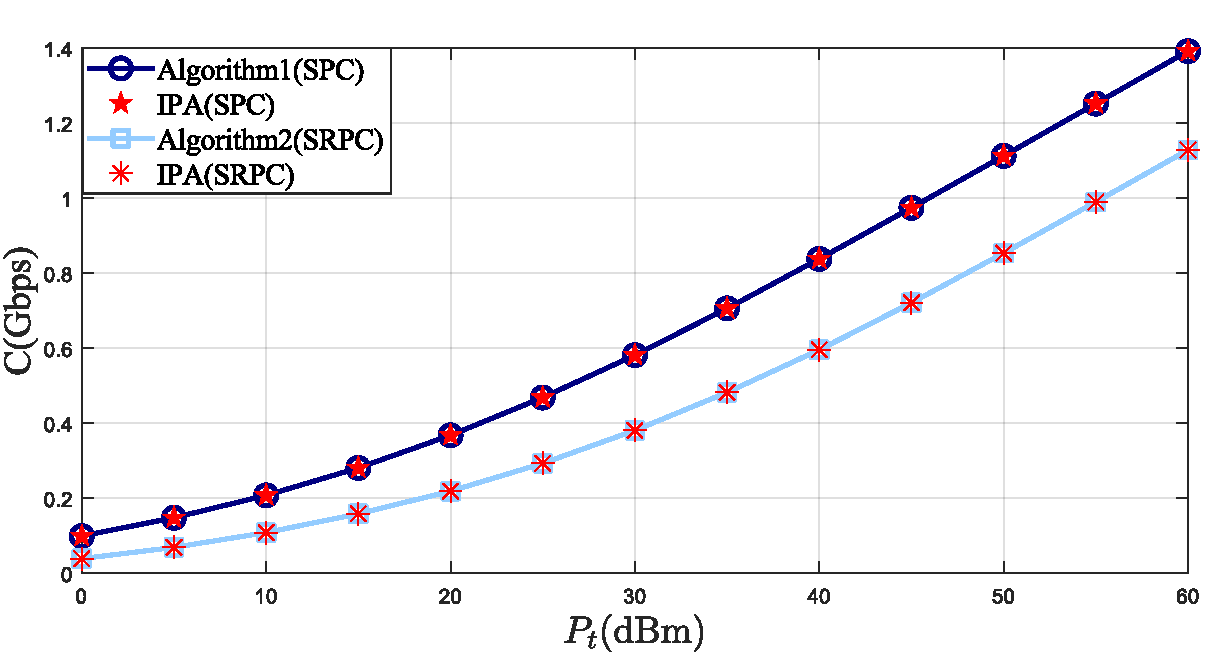
\includegraphics[width=3.5in]{sulv.pdf}
		\caption{Achievable rate of the proposed algorithm under SPC and SRPC (with \( \eta = 0.9 \))}
		\label{fig_sulv}
	\end{figure}
	
	Fig. \ref{fig_sulv} compares the channel capacity under optimal power allocation for both SPC and SRPC, considering four algorithms: Algorithm 1, Algorithm 2, and their corresponding interior-point methods. In the case of SRPC with \( \eta = 0.9 \), the figure highlights the impact of uneven power distribution on SRPC. Note that the interior-point methods for both SPC and SRPC are applied after the optimal subcarrier matching and arrangement. Specifically, for SPC, the interior-point method solves \eqref{eq:7}, and for SRPC, it solves \eqref{eq:separate_power_constraints}.
	
	As shown, the optimal rates obtained by the interior-point methods under both SPC and SRPC match those of Algorithm 1, which confirms Theorems 1 and 3. That is, the extension of the MO theorem to the DH-HPWS (under SPC and SRPC conditions) holds true. This also validates the correctness of our algorithm.
	
	In terms of time complexity, we recorded the execution time of Algorithm~2 and its corresponding interior point method under different power levels, averaged over 1000 trials with \( \eta = 0.5 \), as shown in Table~\ref{tab:compact_twocol}. Here, A2 denotes Algorithm~2. It can be observed that for optimal subcarrier matching, the average runtime of IP-NSM is several times higher than that of A2-NSM, while both achieve nearly the same maximum achievable transmission rate. 
	
	Moreover, the analysis shows that transmit power has little impact on the runtime of the algorithms. In addition, Algorithm~2 with subcarrier matching requires nearly 100 times less computation time compared to the version without subcarrier matching. This significant difference is primarily related to the structural steps of Algorithm~2, and the detailed explanation will be provided in the following sections.
	
	
	
	
	\begin{table*}[htbp]
		\scriptsize % 缩小字体,使表格更紧凑
		\setlength{\tabcolsep}{3pt} % 缩小列间距
		\centering
		\caption{Algorithm Runtime (in seconds)}
		\label{tab:compact_twocol}
		\begin{tabular}{l@{\hspace{3pt}} *{13}{S[table-format=1.2e-1]}}
			\toprule
			\textbf{Pt(dBm)} 
			& \multicolumn{1}{c}{0} & \multicolumn{1}{c}{5} & \multicolumn{1}{c}{10} 
			& \multicolumn{1}{c}{15} & \multicolumn{1}{c}{20} & \multicolumn{1}{c}{25} 
			& \multicolumn{1}{c}{30} & \multicolumn{1}{c}{35} & \multicolumn{1}{c}{40} 
			& \multicolumn{1}{c}{45} \\
			\midrule
			\textbf{IP-NSM [s]} 
			& 2.16e-1 & 2.27e-1 & 2.26e-1 & 2.18e-1 & 2.17e-1 & 2.18e-1 
			& 2.70e-1 & 3.12e-1 & 2.22e-1 & 2.28e-1 \\
			\textbf{A2-NSM [s]} 
			& 1.54e-2 & 1.55e-2 & 1.57e-2 & 1.55e-2 & 1.51e-2 & 1.53e-2 
			& 2.25e-2 & 1.94e-2 & 1.54e-2 & 1.66e-2 \\
			\textbf{A2-OSM [s]} 
			& 2.45e-4 & 1.84e-4 & 1.96e-4 & 1.72e-4 & 1.79e-4 & 1.73e-4 
			& 1.97e-4 & 3.61e-4 & 1.75e-4 & 2.10e-4 \\
			\bottomrule
		\end{tabular}
		
	\end{table*}
	
	
	
	\begin{figure}[!t]
		\centering
		\subfloat[]{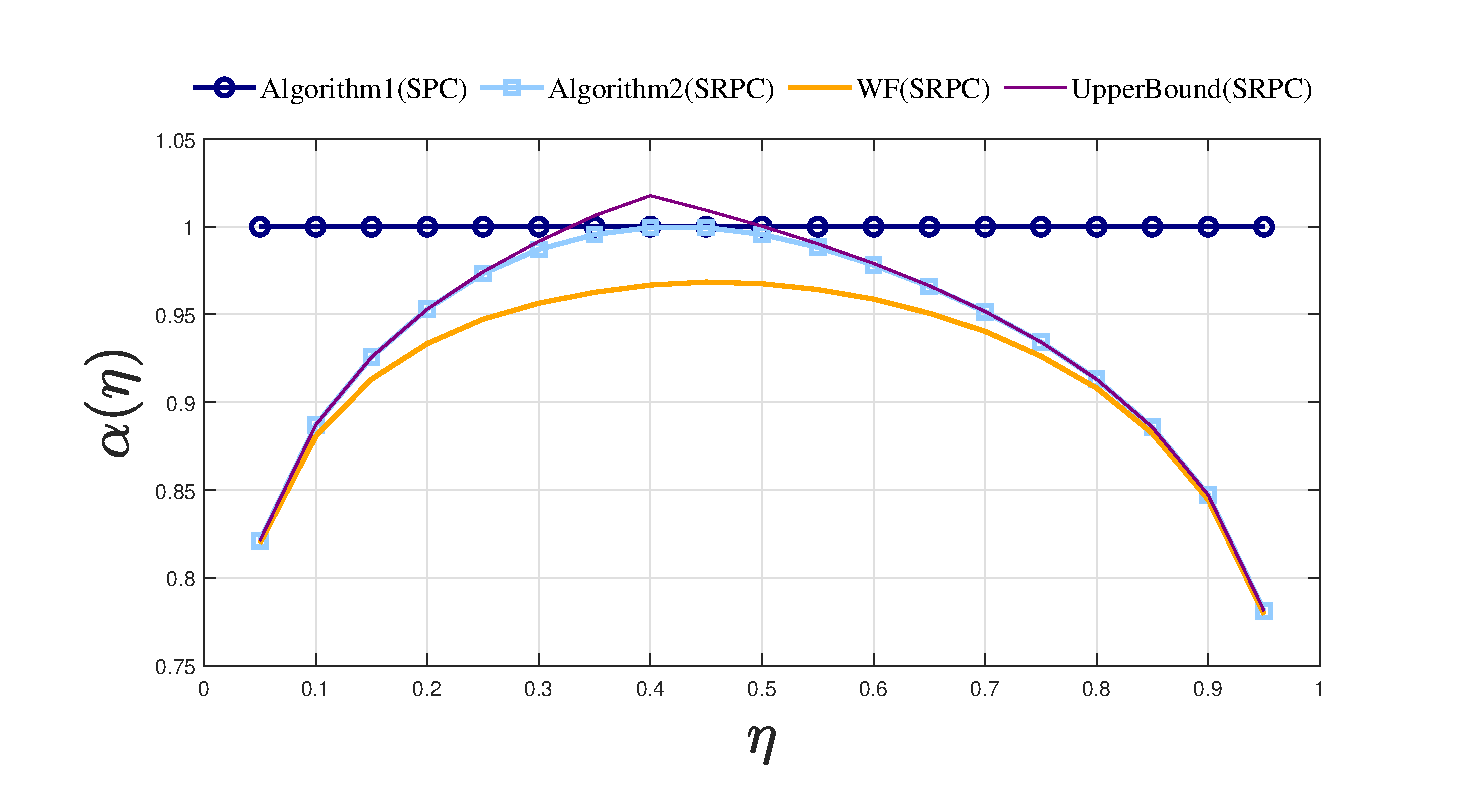
\includegraphics[width=3.3in]{eta_unsort.eps}%
			\label{fig_eta}}
		\hfil
		\subfloat[]{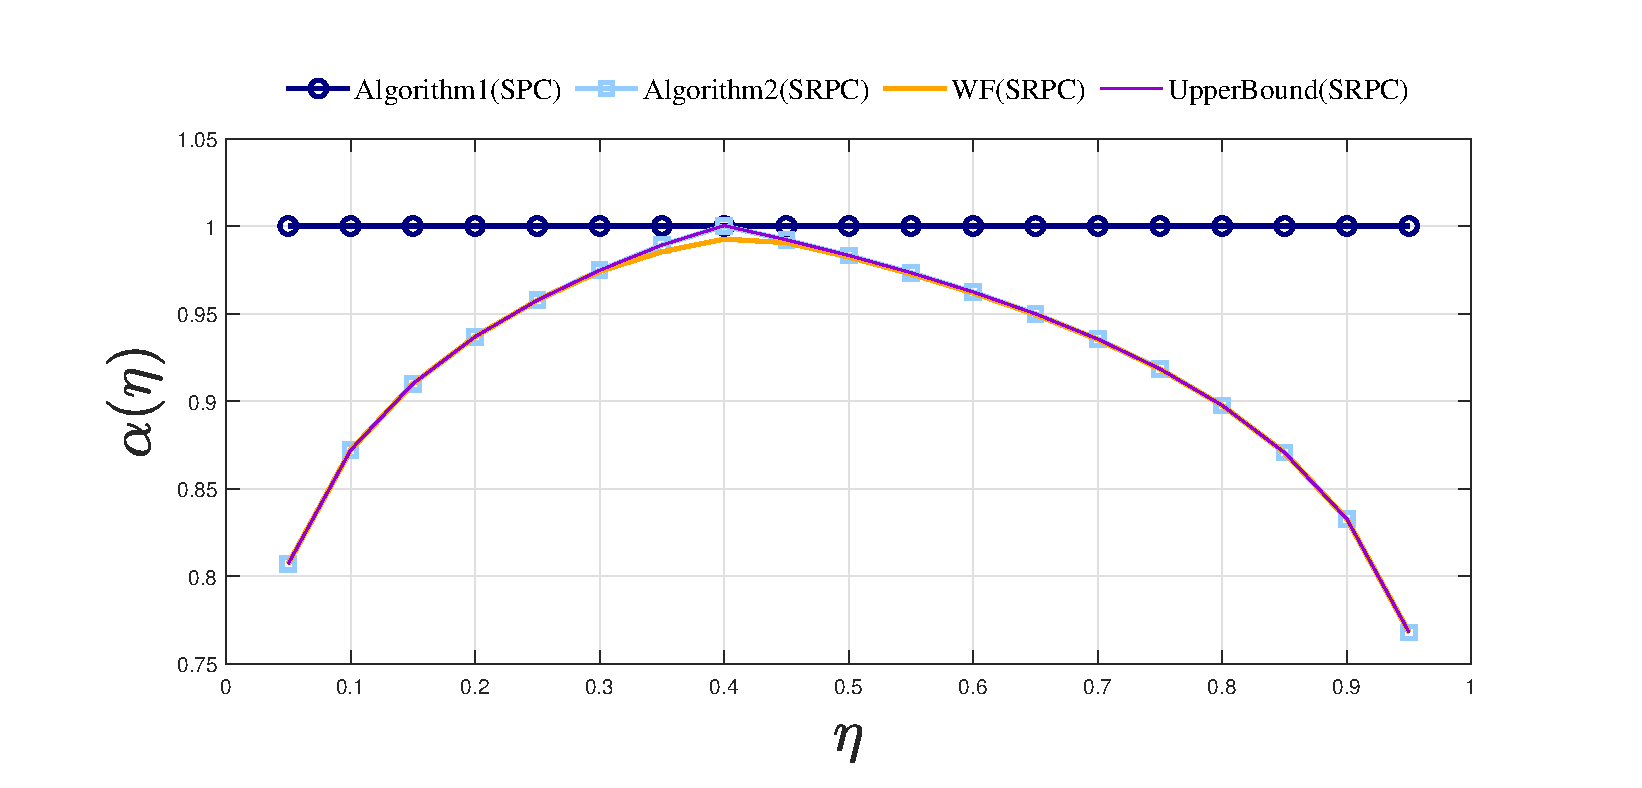
\includegraphics[width=3.3in]{eta_sort.eps}%
			\label{fig_eta_sorted}}
		\caption{Achievable rate ratio of different algorithms versus \( \eta \) for \( P_t = 30 \, \text{dBm} \) for (a) NSM, (b) OSM.}
		\label{fig_eta_all}
	\end{figure}
	
	Fig. \ref{fig_eta_all} shows the relationship between \( \alpha \) and \( \eta \), where \( \eta \in \{0.05, 0.95\} \), and \( \alpha = \frac{C'}{C_A} \), with \( C' \) representing one of the channel capacities computed by the four algorithms in Fig. \ref{fig_eta_all}. These include Algorithm 1 under SPC, Algorithm 2 under SRPC, and the water-filling algorithms at both ends (\(S\) and \(R\)) under SPC and SRPC upper bounds, and \( C_A \) represents the result of Algorithm 1.
	
	
	Note that the "water-filling" at both ends refers to applying the water-filling algorithm after using the MO algorithm to simplify the mixed channels into non-mixed channels and then separately applying the water-filling algorithm at the source and relay ends.
	
	Starting from Fig.  \ref{fig_eta_all}(a), we can observe that the achievable data rate under the SPC constraint is greater than or equal to that under the SRPC constraint. However, the SRPC upper bound, as given by \eqref{eq:15}, can exceed the achievable data rate under the SPC constraint. This result suggests that the maximum achievable rate under the SPC system is not the same as the maximum achievable rate at the source or relay under the SRPC constraint. It also indicates that, in certain cases of \( \eta \), the SRPC upper bound is not achievable.
	
	If both ends consider only their own optimal solution, i.e., the source and relay both use the water-filling algorithm, then the ratio of achievable rates in the DH-HPWS to the achievable rate under SPC is shown by the yellow curve. It is worth noting that the curves of Algorithm 2 and the SRPC upper bound do not overlap, and they only coincide when Algorithm 2 reaches its second phase.
	
	Fig.  \ref{fig_eta_all}(b) shows that the SRPC upper bound does not exceed the achievable data rate under SPC, and it coincides with the curve of Algorithm 2. This indicates that the achievable data rate under SRPC is equal to the SRPC upper bound. In other words, Algorithm 2 only operates in the first phase and returns without executing the second, more complex phase, resulting in significantly reduced execution time.
	
	Moreover, for certain values of \( \eta \), the achievable data rate of Algorithm 2 matches that of the waterfilling algorithm applied separately at both ends. Even when the achievable rates differ, the discrepancy is less than 5\%. This demonstrates that when the source and relay separately execute the waterfilling algorithm, the rate of each subchannel at the source is greater than that of the matching subchannel at the relay. However, this overlap is nearly nonexistent in Fig. \ref{fig_eta_all}(a).
	
	In conclusion, optimal subcarrier matching greatly enhances the efficiency of Algorithm 2. When optimal matching is used, the near-optimal method, where the waterfilling algorithm is executed separately at both ends, can replace Algorithm 2. This approach simplifies the system by requiring only the source and relay to know their own CSI, without the need for the relay to know the CSI of both time slots.
	
	\begin{figure}[!t]
		\centering
		\subfloat[]{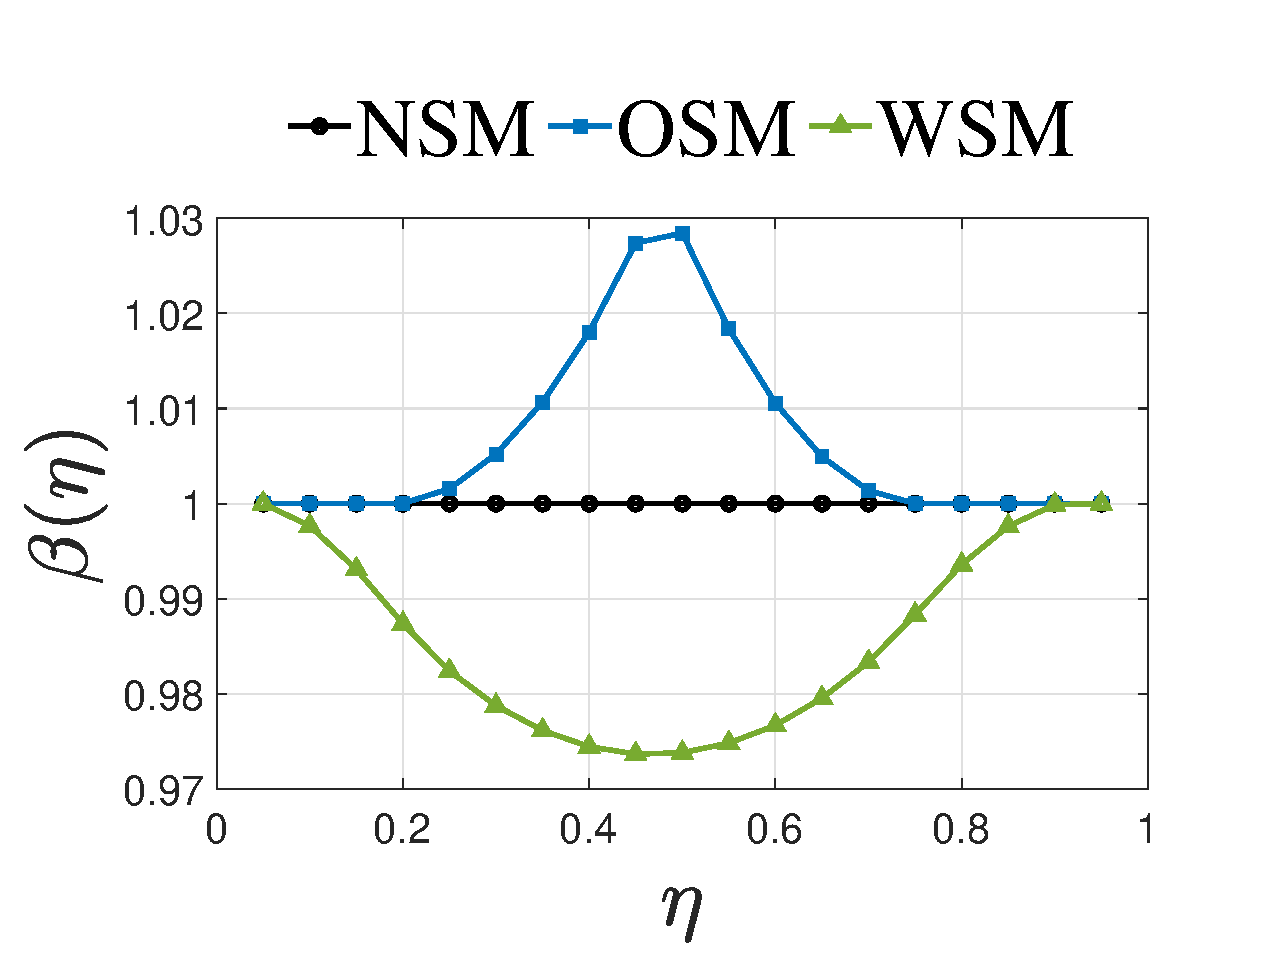
\includegraphics[width=0.24\textwidth]{OSM.eps}%
			\label{fig_beta}}
		\hfil
		\subfloat[]{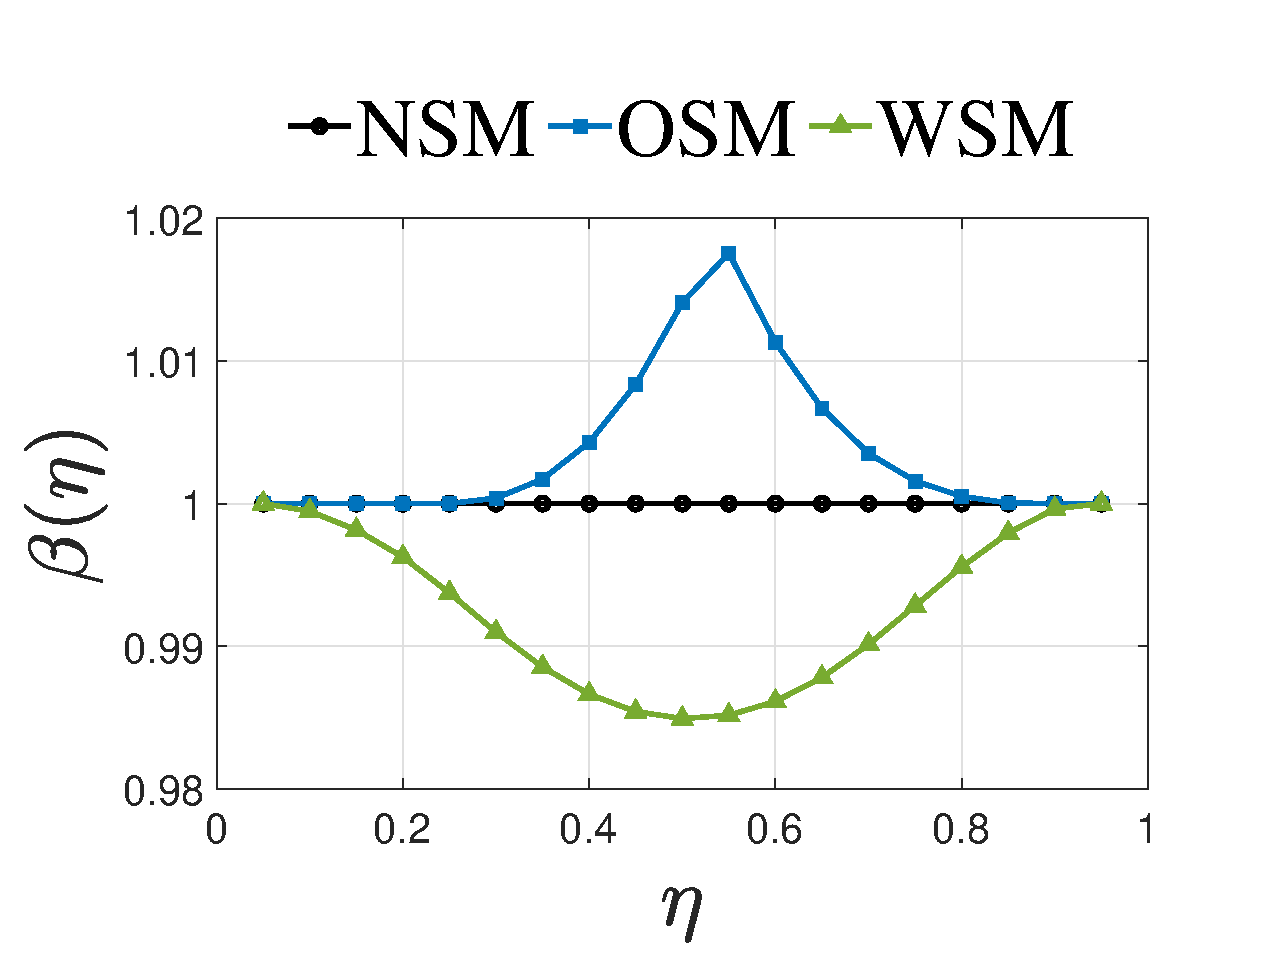
\includegraphics[width=0.24\textwidth]{OSM_20.eps}%
			\label{fig_beta_20}}
		\caption{The gain brought by subcarrier matching under SPC for different values of \( \eta \) for (a) \( P_t = 0 \, \text{dBm} \). (b) \( P_t = 20 \, \text{dBm} \).}
		\label{fig_beta_all}
	\end{figure}
	
	Turning to Fig. \ref{fig_beta_all}, we define \( \beta \buildrel \Delta \over = \frac{C_\xi}{C_{NSM}} \) to represent the gain ratio that can be achieved by subcarrier matching. Analyzing the data, it is clear that OSM provides higher data rates than NSM or WSM. At \( P_t = 0 \, \text{dBm} \) and \( P_t = 20 \, \text{dBm} \), the maximum gain can reach approximately 4\% and 2\%, respectively. Notably, the OSM curve is steeper than the WSM curve, and for small or large values of \( \eta \), OSM and NSM provide the same achievable data rate. This is because, when \( \eta \) is small (or large), both the \(S\) and \(R\) in the OSM and NSM cases can satisfy the waterfilling algorithm for each other. Additionally, these values indicate that as \( P_t \) increases, the gain from subcarrier matching decreases.
	
	\section{Conclusion}
	\label{conl}
	This paper investigates the power allocation problem in the DH-HPWS, providing a system model under the assumption of OFDM and MRC. A mathematical analysis of the optimal power allocation problem is conducted, and an optimal power allocation algorithm under the SPC and SRPC  is proposed to maximize the system channel capacity. The obtained results provide important insights for practical deployment and optimization of DH-HPWS in future communication networks.
	
	For the SRPC, this paper proves that the optimal subcarrier matching pairs high-nSNR channels with high-nSNR channels and low-nSNR channels with low-nSNR channels, which is similar to the optimal subcarrier matching under the SPC constraint \cite{wenyi2008}. Interestingly, the subcarrier arrangement in the same timeslot is shown to match low-nSNR channels with high-nSNR channels, which is the complete opposite of the subcarrier matching in different timeslots.
	
	Through the IP-based algorithms, we verify the correctness of Theorem 1, 2, and Corollary 1, 2. Numerical analysis shows that our algorithm outperforms the traditional waterfilling algorithm. Additionally, the results indicate that using OSM provides numerous benefits, including reducing algorithm time complexity, improving the achievable rate of the DH-HPWS, and simplifying the communication process.
	
	
	\section*{Appendix A}
	\begin{lemma}[Two-subcarrier OFDM case]
		Under optimal subcarrier pairing, within the same equivalent medium, the subcarrier with higher nSNR always achieves a higher rate than the one with lower nSNR.
	\end{lemma}
	\begin{proof}
		See Lemma 1 in \cite{5071270}.
	\end{proof}
	\begin{corollary}
		Under optimal power allocation at the \(S\), in order to satisfy rate equality, the power required at the R node for pairing a high-nSNR channel with another high-nSNR channel is less than that required for pairing a high-nSNR channel with a low-nSNR channel.
	\end{corollary}
	\begin{proof}
		Assuming that under the pairing of a high-nSNR channel with a low-nSNR channel, both \( S \) and \( R \) achieve optimal power allocation. According to Lemma 1, when a high-nSNR channel is paired with another high-nSNR channel, there exists a power allocation at \( R \) such that the rates of its two subchannels are individually greater than those of the corresponding subchannels at \( S \). Therefore, the power at \( R \) can be reduced so that the rate of each subchannel at \( R \) equals that of its matched subchannel at \( S \).
	\end{proof}
	According to the corollary, the relationship between \( P_S \) and \( P_R \) can be categorized into three cases:
	
	1) Under suboptimal pairing, if \( P_R \) is sufficiently large, it can support the water-filling power allocation strategy at the \( S \) node, and the channel capacity reaches its upper bound.  Under this condition, channel pairing has no impact on maximizing the system's achievable rate.
	
	
	2) Under suboptimal pairing, if \( P_R \) cannot support the water-filling power allocation strategy at the \( S \) node, but under optimal pairing, \( P_R \) can support it. Under this condition, since it is evident that suboptimal pairing cannot reach the upper bound, the achievable rate under optimal pairing is higher.
	
	3) Even under optimal pairing, \( P_R \) cannot support the water-filling power allocation strategy at the \( S \) node.Under this condition, the achievable rate under optimal pairing is higher. The proof is as follows:
	\begin{proof}
		Assume that the OFDM system over the equivalent medium at both the \( S \) and \( R \) nodes has two subcarriers, denoted by \( \overline{\gamma}_{\mathrm{SR}}^1, \overline{\gamma}_{\mathrm{SR}}^2, \overline{\gamma}_{\mathrm{RD}}^1, \overline{\gamma}_{\mathrm{RD}}^2 \), where \( \overline{\gamma}_{\mathrm{SR}}^1 \le \overline{\gamma}_{\mathrm{SR}}^2 \) and \( \overline{\gamma}_{\mathrm{RD}}^1 \le \overline{\gamma}_{\mathrm{RD}}^2 \). Suppose that the subchannel with higher nSNR at the \( S \) node is paired with the subchannel with lower nSNR at the \( R \) node. Assume optimal power allocation has been performed to maximize the overall achievable rate. In this case, we have \( R_{SR}^1 = R_{RD}^2 \) and \( R_{SR}^2 = R_{RD}^1 \), and thus the achievable system rate is \( R_{SR}^1+R_{SR}^2 \).
		
		According to \textbf{Lemma 1}, there exists a new power allocation at the \( R \) node such that \( R_{RD}^{1'} > R_{RD}^{2} \) and \( R_{RD}^{2'}> R_{RD}^{1} \), i.e., \( R_{RD}^{1'} > R_{SR}^{1} \) and \( R_{RD}^{2'} > R_{SR}^{2} \). After swapping the subcarrier pairing order at the \( R \) node and the \( S \) node and applying the new power allocation scheme, since this is the third case, the power allocation at the \( S \) node, \( P_{S,1} \) and \( P_{S,2} \), is not optimal. We move the power allocation toward the optimal distribution until \(  R_{SR}^{1'} =  R_{RD}^{1'} \) and \(  R_{SR}^{2'} = R_{RD}^{2'} \). At this point, the total system capacity becomes \(  R_{SR}^{1'} +R_{SR}^{2'} > R_{SR}^{1} + R_{SR}^{2} \). This proves that pairing high-nSNR subcarriers with high-nSNR subcarriers leads to a higher achievable channel capacity.
		
	\end{proof}
	
	
	
	
	\section*{Appendix B}
	
	Similarly, we assume that \( \hat{R}_{SR} < \hat{R}_{RD} \), and all propositions in Appendix B are made under the assumption of the second scenario. Note that Proposition 1 is the default.
	\begin{lemma}
		 If \( P_R \) does not satisfy the \(S\) water-filling condition, neither the \(S\) end nor the \(R\) end satisfies their individual optimal power distribution.
	\end{lemma}
	
	\begin{proof}
		
		1. The node \(R\) cannot satisfy the condition. According to \eqref{eq:15}, the system's achievable rate upper bound \({C_{up}} = \hat {R}_{SR}\). If node \(R\) satisfies the independent optimal power allocation, the system's achievable rate becomes \(\hat {R}_{RD} > {C_{up}}\).
		
		2. The  node \(S\) cannot be satisfied. The second case is determined by the constraints.
	\end{proof}	
	\subsection*{Proposition for the case when \( N = 2 \).}
	The content of this section assumes \( N = 2 \), meaning that the number of subchannels for the equivalent medium is 2.
	
	\begin{lemma}[Two-subcarrier OFDM case]
		When the optimal power allocation is satisfied, as the \(S\) moves towards its independent optimal direction, the required power at the \(R\) increases to maintain equal channel rates with the \(S\).
	\end{lemma}
	\begin{proof}
		If there is no increase, the DH-HPWS achieves a higher rate, indicating that the power allocation is suboptimal.
	\end{proof}	
	\begin{proposition}[Two-subcarrier OFDM case]
		 If \( P_R \) does not satisfy the \(S\) water-filling condition, there is no power surplus under the overall optimal power allocation of the system.
	\end{proposition}
	\begin{proof}
		First, it is impossible for both \(S\) and \(R\) to simultaneously have a power surplus. If such a surplus exists, allocating the excess power to the same matched subchannel can achieve a higher achievable rate, indicating that the power allocation is not optimal.  
		Second, by Lemma 1, assuming the \(R\) end has a power surplus, the power at the \(S\) end can be adjusted in the optimal direction, and the surplus power at the R end can be accommodated. Thus, \( R_{SR}' > R_{SR} \), which indicates a suboptimal power allocation, and therefore no power surplus exists. The same reasoning applies if the \(S\) has a power surplus.
	\end{proof}
	This section proves the correctness of Proposition 3 in the case of two subchannels. The next section will generalize this Proposition to \( N \) subchannels.
	\subsection*{Proposition under \( N \) subchannels}
	This section generalizes Proposition 3 to the case of \( N \) subchannels.
	\begin{lemma}
		The optimal power allocation for any two channels implies the optimal power allocation for \( N \) channels.
	\end{lemma}
	\begin{proof}
		Due to the length limitation of the article, the proof is omitted.
	\end{proof}
	\begin{corollary}
		Proposition 3 still holds under \( N \) subchannels.
	\end{corollary}
	\begin{proof}
		In the second scenario, based on Lemma 1 and the contrapositive of Lemma 3, we have: there exist two channels where the power allocation is not independently optimal. According to Proposition 3, a power surplus cannot exist. Thus, the proof is completed.
	\end{proof}
	
	
\bibliographystyle{IEEEtran}
\bibliography{references}

\end{document}




